
\chapter{Design}
\renewcommand{\chaptername}{Chapter}


~~~~~In order to reach the appropriate result as described in the specifications, we need to clarify the
project main architecture, as well as the architecture of its components.

This chapter focuses on designing a suitable structure for the application. This step is crucial in the course of the project and aims to undertake and prepare the ground for the implementation phase.

\section{Physical architecture}
In this section, we briefly study the proposed architecture to make sure it is corresponding to the goals of the project.

Figure \ref{physic_arch} presents the physical architecture of our solution in ATHENA's network. In the following paragraphs, we describe each component of the architecture and the corresponding role.

\begin{itemize}
    \item \textbf{RITA:}
    
    Real Threat Intelligence Analysis is used as our threat intelligence platform, pulling Bro logs from our SecurityOnion Box for later analysis.
    \item\textbf{SecurityOnion Standalone box:} 
    
    This box is an instance of SecurityOnion along with its tools to sniff ATHENA's in and out traffic and run it through Intrusion Detection Systems(Suricata and Bro), correlate events and alerts for later use. It is connected directly to the switch with a port mirroring option(used on a network switch to send a copy of network packets seen on one switch ports).
    \begin{figure}[!htpb] 
    \begin{center}
    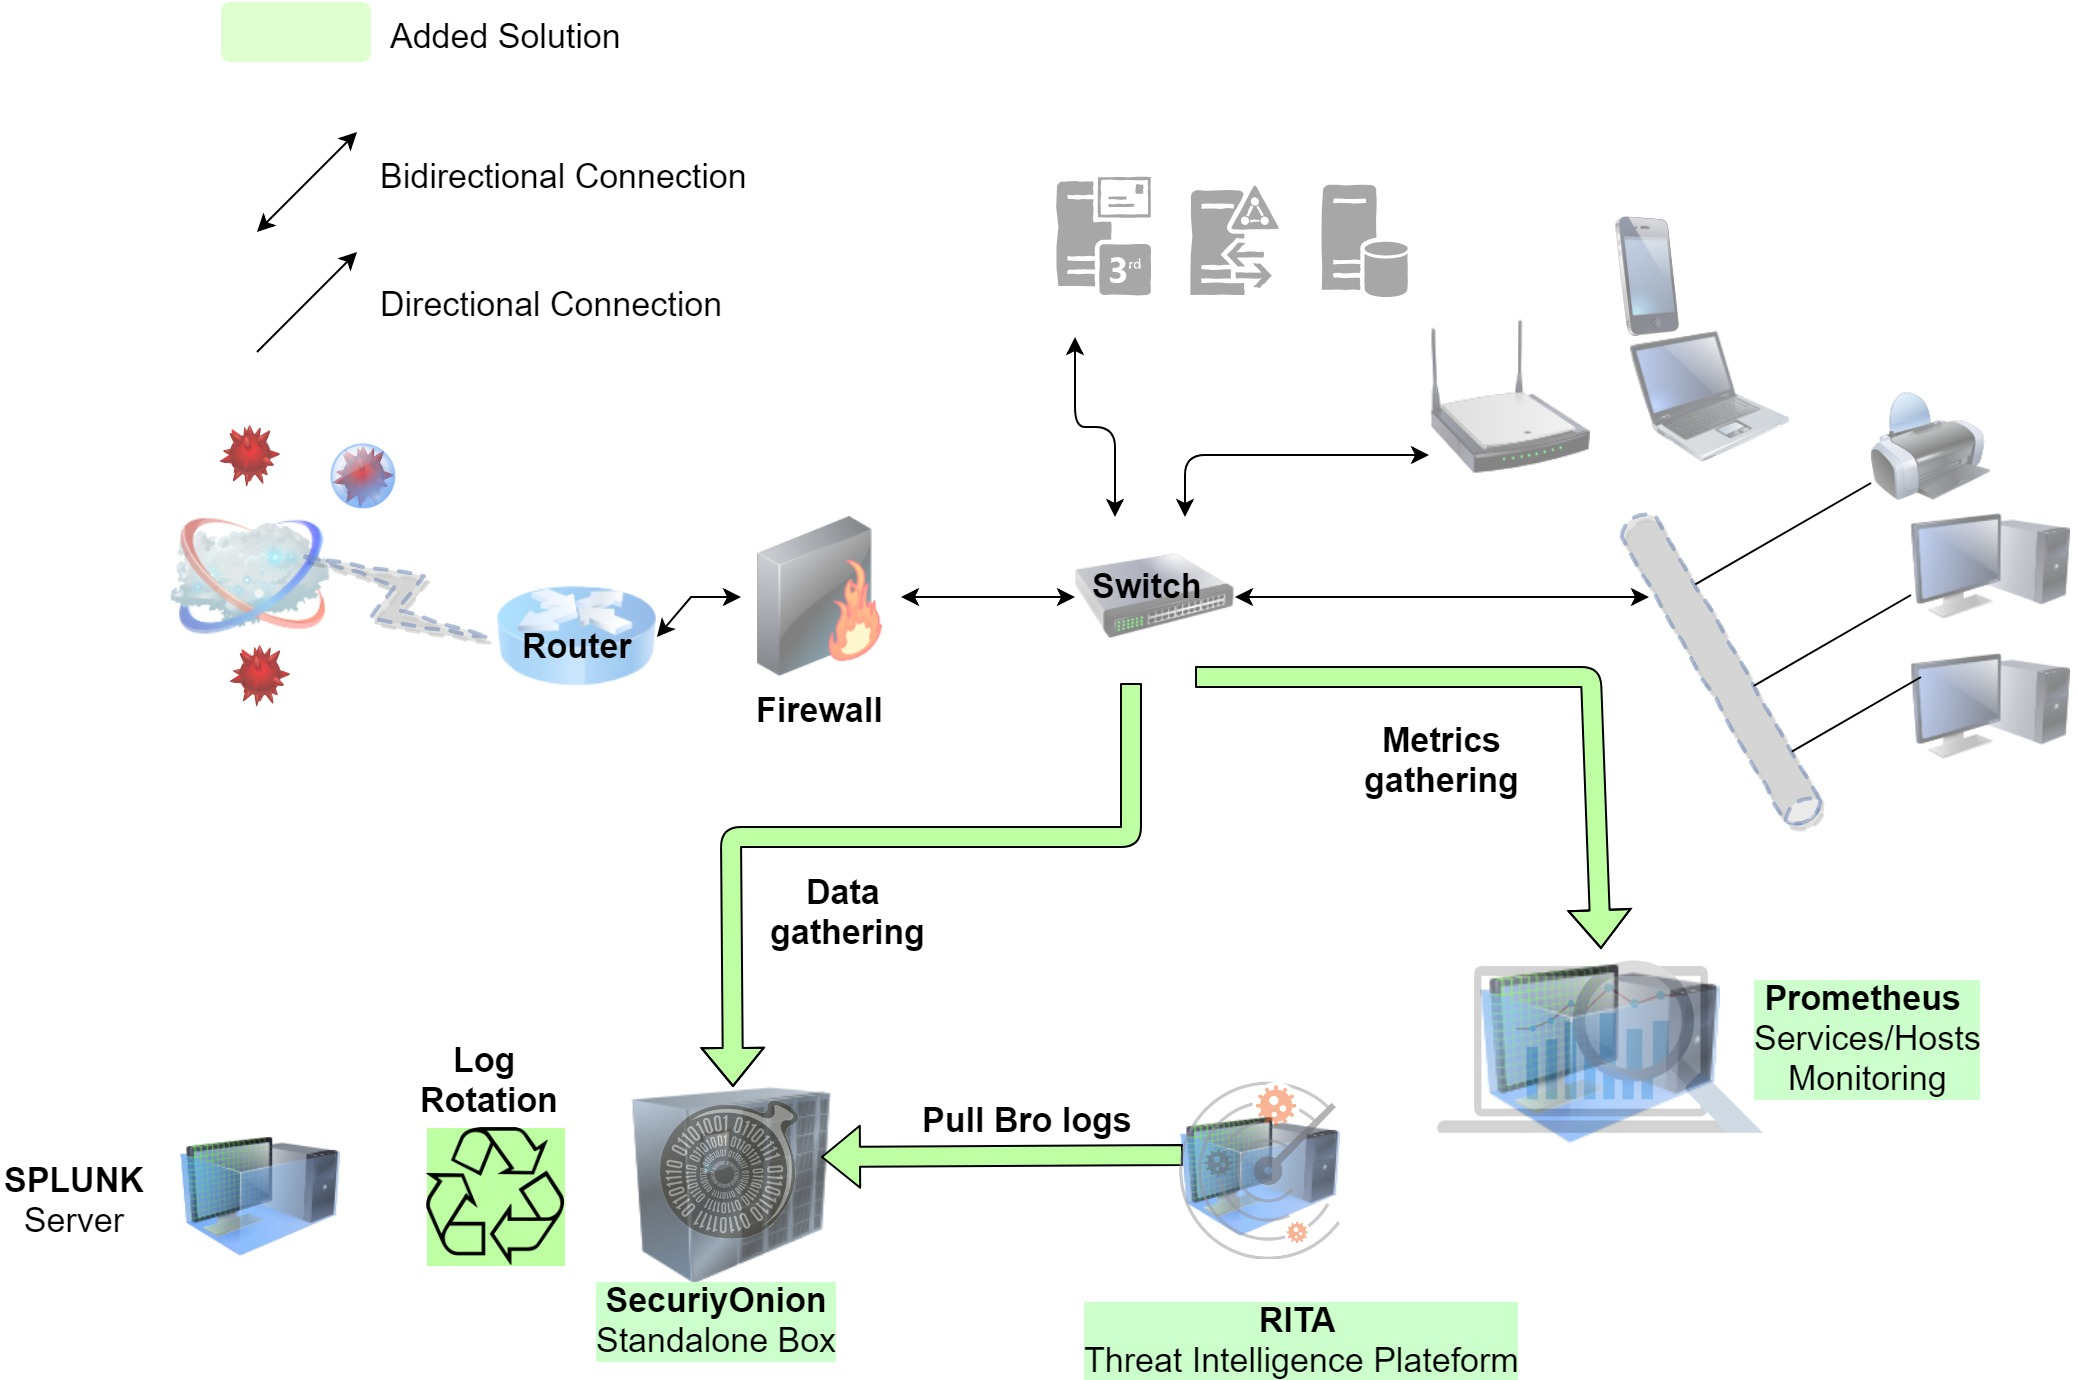
\includegraphics[width=6.3 in]{images/ATHENANewNetworkarch.jpg}
    \caption{Physical Architecture}
    \label{physic_arch}
    \end{center}
    \end{figure}~
    \item\textbf{SPLUNK Server:}
    
    SPLUNK server is already is already implemented in ATHENA, so we are going to use it in the log-rotation process(an automated process used in system administration in which dated log files are archived).
    \item \textbf{Prometheus Server:}
    
    It is a monitoring system and time series database. Placed to receive or gather metrics(internationally adopted decimal system.)
    \item \textbf{ATHENA's Endpoints:}
    
    Servers and workstations running different operating systems. Configured to send metrics to provide detailed information about system or services activity to Prometheus Server.
\end{itemize}




\section{Logical architecture}

In order to plan and understand the global design of our project, a detailed logical architecture is necessary. whose purpose is to achieve a clean separation between the components.

\subsection{SecurityOnion Box}

Figure \ref{logic_archso} illustrate SecurityOnion's main components interactions. The next paragraphs represents those components and their relations :

\begin{itemize}
    \item\textbf{Intrusion detection systems } 
    
    Network and Host IDS are placed on the bottom as they represent the first layer that is responsible for detection and alert generation based on configurable rules and scrips. Network IDS are receiving data on the network from a tool called Netsniff-ng, Host based IDS pulls processes and host activity logs from Sysmon and OSSEC agents or Syslog servers placed in Endpoint workstations or servers.
    \item\textbf{ElasticSllaearch-Logstash-Kibana }
    
    The Elastic stack is the combination of Logstash, Elasticsearch, Kibana responsible respectively of index, storage/search and visualisation of alerts and events. Curator helps Elasticsearch organise indices, Elastalert help manage alerts over the time.
    \item\textbf{Docker systems }
    
    It is a software-as-a-service tool that enables users to publish and share container-based applications through a common library. The Elastic Stack in our solution is deployed in containers and docker images.
\end{itemize} 
\begin{figure}[!htpb] 
\begin{center}
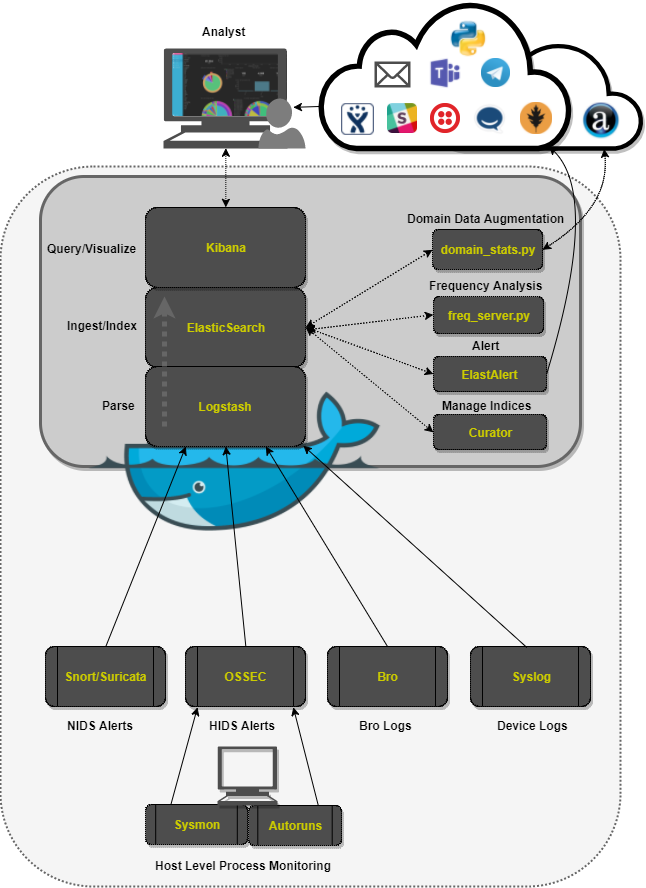
\includegraphics[width=6.3 in]{images/best_arch_so_far.png}
\caption{SecurityOnion Logical Architecture}
\label{logic_archso}
\end{center}
\end{figure}~

\newpage
\subsection{Prometheus Server}
Figure \ref{logic_archpro} illustrate metrics monitoring server's main components interactions. The next paragraphs represents those components and their relations :


\begin{figure}[!htpb] 
\begin{center}
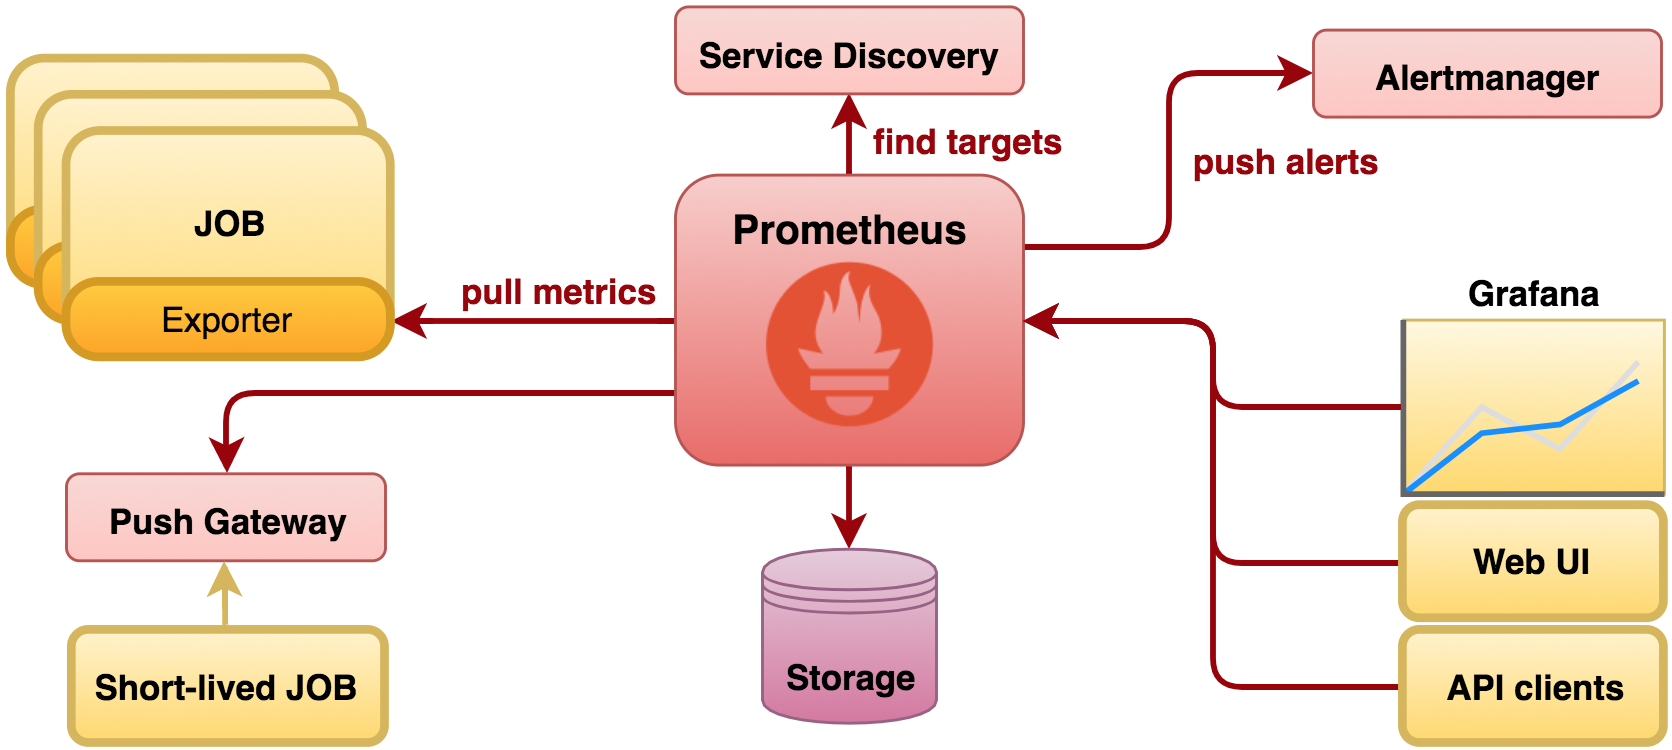
\includegraphics[width=6.0 in]{images/ATHENAprom-arch.png}
\caption{Prometheus's Logical Architecture}
\label{logic_archpro}
\end{center}
\end{figure}~

\begin{itemize}
    \item\textbf{Prometheus:}
    
    Prometheus is an open-source monitoring system with a dimensional data model, flexible query language, efficient time series database and modern alerting approach. Targets (it can be services or jobs) are registered to export metrics to Prometheus, Prometheus comes with a configurable Alertmanager responsible for user's notification in case of failures.
    \item\textbf{Grafana:}
    
    We are using Grafana as the data visualization and monitoring with support for Prometheus. Prometheus's gathered metrics are visualized in graphs and tables with Grafana.
\end{itemize}
%------------------------------------------------





\subsection *{Conclusion}
Through this chapter, we displayed the general architecture of our application. We explained subsequently the choice of our logical and physical architecture. In the next chapter, we present and expose the technologies employed during the process of creating our toolkit along with the added functionalities.

